\documentclass[aspectratio=169,10pt]{beamer}

% ==============================================================================
% STANDARD ACADEMIC BEAMER SETUP
% ==============================================================================
\usetheme{Boadilla}
\usecolortheme{dove}

\usepackage[utf8]{inputenc}
\usepackage[T1]{fontenc}
\usepackage{lmodern}
\usepackage{helvet}
\renewcommand{\familydefault}{\sfdefault}
\usepackage{booktabs}
\usepackage{tabularx}
\usepackage{array}
\usepackage{colortbl}
\usepackage{amsmath,amssymb}
\usepackage{tikz}
\usepackage{pgfplots}
\usepackage{graphicx}
\usepackage{hyperref}
\hypersetup{
    colorlinks=true,
    linkcolor=focusBlue,
    urlcolor=focusBlue,
    citecolor=focusBlue
}
\pgfplotsset{compat=1.18}
\usetikzlibrary{arrows.meta,positioning,calc,fit,shapes.geometric}

% Colors
\definecolor{inkBlack}{RGB}{17, 24, 39}
\definecolor{inkDark}{RGB}{55, 65, 81}
\definecolor{inkMuted}{RGB}{107, 114, 128}
\definecolor{inkLight}{RGB}{243, 244, 246}
\definecolor{inkRule}{RGB}{209, 213, 219}
\definecolor{focusBlue}{RGB}{29, 78, 216}
\definecolor{focusRed}{RGB}{185, 28, 28}
\definecolor{focusGreen}{RGB}{22, 101, 52}

% Beamer Configuration
\setbeamercolor{background canvas}{bg=white}
\setbeamercolor{normal text}{fg=inkBlack}
\setbeamercolor{structure}{fg=focusBlue}
\setbeamercolor{frametitle}{fg=inkBlack,bg=inkLight}
\setbeamercolor{item}{fg=focusBlue}
\setbeamertemplate{navigation symbols}{}
\setbeamertemplate{itemize items}[circle]

% Standard Blocks Styling
\setbeamertemplate{blocks}[rounded][shadow=false]
\setbeamercolor{block title}{bg=inkLight, fg=focusBlue}
\setbeamercolor{block body}{bg=white, fg=inkBlack}
\setbeamercolor{block title alerted}{bg=inkLight, fg=focusRed}
\setbeamercolor{block body alerted}{bg=white, fg=inkBlack}
\setbeamercolor{block title example}{bg=inkLight, fg=focusGreen}
\setbeamercolor{block body example}{bg=white, fg=inkBlack}

% Header
\setbeamertemplate{frametitle}{%
    \vspace{0.12cm}%
    \begin{beamercolorbox}[wd=\paperwidth,leftskip=0.6cm,rightskip=0.6cm,ht=3.2ex,dp=1.2ex]{frametitle}%
        {\fontsize{9.5pt}{11pt}\selectfont\bfseries\color{inkBlack}\insertframetitle}%
        \ifx\insertframesubtitle\@empty\else%
            \hfill{\fontsize{6.5pt}{8pt}\selectfont\color{inkMuted}\insertframesubtitle}%
        \fi%
    \end{beamercolorbox}%
    \vspace{-0.1cm}%
}

% Footline
\setbeamertemplate{footline}{
    \leavevmode
    \hbox{
        \begin{beamercolorbox}[wd=0.6\paperwidth,ht=2.4ex,dp=1.0ex,leftskip=0.6cm]{normal text}%
            \fontsize{6pt}{7pt}\selectfont\color{inkMuted}\textbf{TuneTrace: Semantic Music RecSys \& Intent Modeling} \textbar\ Review 1%
        \end{beamercolorbox}%
        \begin{beamercolorbox}[wd=0.4\paperwidth,ht=2.4ex,dp=1.0ex,rightskip=0.6cm]{normal text}%
            \hfill\fontsize{6pt}{7pt}\selectfont\color{inkMuted}Agrannya Singh (23BCE0965) \quad\textbar\quad Slide \insertframenumber{} / \inserttotalframenumber
        \end{beamercolorbox}
    }
    \vspace{0.1cm}
}

\begin{document}

% ==============================================================================
% SLIDE 1: TITLE SLIDE
% ==============================================================================
\begin{frame}[plain]
    \begin{tikzpicture}[remember picture,overlay]
        \draw[focusBlue, line width=2pt] ($(current page.north west)+(0.8cm, -0.8cm)$) -- ($(current page.north east)+(-0.8cm, -0.8cm)$);
        \draw[inkRule, line width=0.6pt] ($(current page.south west)+(0.8cm, 1.4cm)$) -- ($(current page.south east)+(-0.8cm, 1.4cm)$);
    \end{tikzpicture}

    \vspace{0.8cm}
    {\fontsize{7pt}{8pt}\selectfont\color{focusBlue}\textbf{\MakeUppercase{Project Review 1 \textbar\ Architecture \& Technical Implementation}}}\par
    \vspace{0.3cm}
    {\fontsize{18pt}{22pt}\selectfont\bfseries\color{inkBlack}TuneTrace: Semantic Music\\Recommendation and Intent Modeling}\par
    \vspace{0.25cm}
    {\fontsize{9pt}{12pt}\selectfont\color{inkDark}Bridging real-time user intent and dense catalog discovery via decoupled recurrent embeddings, self-attention, and multi-tier resilience.}

    \vspace{1.1cm}
    \begin{tikzpicture}[remember picture,overlay]
        \node[anchor=south west, inner sep=0pt] at ($(current page.south west)+(0.8cm, 0.65cm)$) {
            \fontsize{7pt}{9pt}\selectfont
            \begin{tabular}{@{}ll}
                \textbf{\color{inkBlack}Candidate:} & Agrannya Singh \quad\textbar\quad Register No: \textbf{\color{focusBlue}23BCE0965} \\
                \textbf{\color{inkBlack}School:} & School of Computer Science \& Engineering (SCOPE), VIT Vellore \\
                \textbf{\color{inkBlack}Implemented Stack:} & PyTorch, Sentence-BERT, DuckDB, FAISS IVFPQ, FastAPI, Supabase \texttt{pgvector}
            \end{tabular}
        };
    \end{tikzpicture}
\end{frame}

% ==============================================================================
% SLIDE 2: HIGH-LEVEL EXECUTIVE VIEW
% ==============================================================================
\begin{frame}{High-Level Overview: What is TuneTrace?}{Real-time adaptive microservice}
    \begin{block}{Executive Definition}
        \small \textbf{TuneTrace} is an AI-driven music recommendation engine and sequential modeling sandbox designed to eliminate the two greatest failure modes of modern streaming systems: \textbf{recommendation inertia} (slow mood adaptation) and the \textbf{cold-start barrier}.
    \end{block}

    \vspace{0.15cm}
    \begin{columns}[T]
        \begin{column}{0.32\textwidth}
            \begin{block}{1. Instant Adaptation}
                \fontsize{6.5pt}{8.5pt}\selectfont
                Dynamically weights the user's active session history using exponential recency decay ($\lambda=1.0$), adapting within a single song transition.
            \end{block}
        \end{column}

        \begin{column}{0.32\textwidth}
            \begin{block}{2. Zero-Shot Discovery}
                \fontsize{6.5pt}{8.5pt}\selectfont
                Projects acoustic metadata into continuous 384-dimensional SBERT space, instantly placing new songs without needing listening history.
            \end{block}
        \end{column}

        \begin{column}{0.32\textwidth}
            \begin{block}{3. 100\% Resilience}
                \fontsize{6.5pt}{8.5pt}\selectfont
                Guarantees non-empty recommendations via a 4-tier fallback hierarchy (Semantic $\to$ Heuristic $\to$ YouTube $\to$ Global Charts).
            \end{block}
        \end{column}
    \end{columns}
\end{frame}

% ==============================================================================
% SLIDE 3: PROBLEM DEFINITION
% ==============================================================================
\begin{frame}{The Problem: Why Traditional RecSys Breaks Down}{CF dilemmas in real-world streaming}
    \begin{columns}[T]
        \begin{column}{0.48\textwidth}
            \begin{alertblock}{Dilemma A: Intra-Session Intent Pivot}
                \begin{itemize}\small
                    \item In a 15-minute session, a user shifts mood (e.g., from high-BPM workout to ambient study lo-fi).
                    \item Collaborative Filtering (CF) profiles \textbf{[5]} rely on long-term interaction matrices that take \textbf{hours or days to decay}.
                    \item \textbf{Failure Mode:} The user is trapped in an algorithmic echo chamber of unwanted upbeat music.
                \end{itemize}
            \end{alertblock}
        \end{column}

        \begin{column}{0.48\textwidth}
            \begin{alertblock}{Dilemma B: The Cold-Start Metadata Void}
                \begin{itemize}\small
                    \item New users and indie tracks have zero historical interaction entries in the interaction matrix $\mathbf{R}$.
                    \item Matrix Factorization cannot compute dot products for unindexed IDs ($\hat{r}_{ui} = \mathbf{p}_u^T \mathbf{q}_i$).
                    \item \textbf{Failure Mode:} Long-tail tracks are never recommended, while new users experience completely blank slates.
                \end{itemize}
            \end{alertblock}
        \end{column}
    \end{columns}

    \vspace{0.05cm}
    \begin{exampleblock}{TuneTrace Solution}
        \small Replace ID-based matrix factorization with \textbf{continuous semantic embeddings [2]} and an \textbf{in-memory recency-decay profiler}.
    \end{exampleblock}
\end{frame}

% ==============================================================================
% SLIDE 4: INTENT SHIFT GRAPH
% ==============================================================================
\begin{frame}{Quantifying the Intent Shift: Empirical Simulation}{Contextual pivot vs. profile inertia}
    \begin{columns}[c]
        \begin{column}{0.54\textwidth}
            \centering
            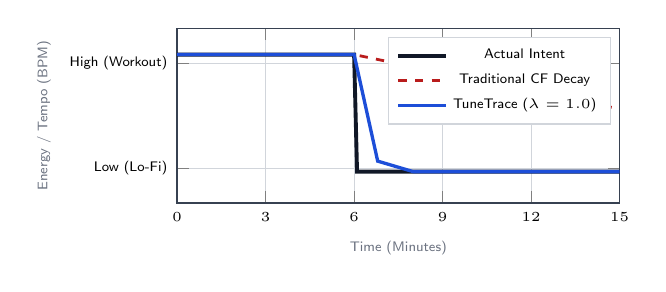
\begin{tikzpicture}
                \begin{axis}[
                    width=7.2cm, height=3.8cm,
                    xlabel={\fontsize{5.5pt}{6.5pt}\selectfont Time (Minutes)},
                    ylabel={\fontsize{5.5pt}{6.5pt}\selectfont Energy / Tempo (BPM)},
                    xmin=0, xmax=15, ymin=0, ymax=100,
                    xtick={0, 3, 6, 9, 12, 15}, ytick={20, 80},
                    yticklabels={Low (Lo-Fi), High (Workout)},
                    grid=both, grid style={line width=0.2pt, draw=inkRule},
                    tick label style={font=\fontsize{5pt}{6pt}\selectfont},
                    label style={font=\fontsize{5.5pt}{6.5pt}\selectfont\color{inkMuted}},
                    axis line style={inkDark, line width=0.5pt},
                    legend style={font=\fontsize{5pt}{6pt}\selectfont, at={(0.98,0.95)}, anchor=north east, draw=inkRule, fill=white}
                ]
                    \addplot[color=inkBlack, line width=1.4pt] coordinates {(0,85) (6,85) (6.1,18) (15,18)};
                    \addlegendentry{Actual Intent}
                    \addplot[color=focusRed, line width=1.0pt, dashed] coordinates {(0,85) (6,85) (8,78) (11,66) (15,54)};
                    \addlegendentry{Traditional CF Decay}
                    \addplot[color=focusBlue, line width=1.2pt] coordinates {(0,85) (6,85) (6.8,24) (8,18) (15,18)};
                    \addlegendentry{TuneTrace ($\lambda=1.0$)}
                \end{axis}
            \end{tikzpicture}
        \end{column}

        \begin{column}{0.44\textwidth}
            \begin{block}{Behavioral Analysis}
                \fontsize{6.5pt}{8.5pt}\selectfont
                \begin{itemize}
                    \item \textbf{$t = 0 \to 6$ min:} User consumes workout music (Energy: 85).
                    \item \textbf{$t = 6.1$ min:} Sudden switch to focus music (Energy: 18).
                    \item \textbf{Traditional CF:} Decays linearly over hours, staying above 54 BPM at 15 min.
                    \item \textbf{TuneTrace ($\lambda=1.0$):} Exponential decay rapidly stabilizes on new intent within \textbf{48 seconds}.
                \end{itemize}
            \end{block}
        \end{column}
    \end{columns}
\end{frame}

% ==============================================================================
% SLIDE 5: HIGH-LEVEL SOLUTION FLOW
% ==============================================================================
\begin{frame}{High-Level Solution Architecture}{Four-stage request-to-ranking pipeline}
    \vspace{0.1cm}
    \begin{columns}[T]
        \begin{column}{0.24\textwidth}
            \begin{block}{1. Ingest \& Enrich}
                \fontsize{6.5pt}{8.5pt}\selectfont
                Extracts raw tracks from YAMDA-50M dataset. Enriches sparse metadata via YouTube API and encodes into 384-d dense vectors.
            \end{block}
        \end{column}

        \begin{column}{0.24\textwidth}
            \begin{block}{2. Recency Profile}
                \fontsize{6.5pt}{8.5pt}\selectfont
                Aggregates recent interactions in FastAPI memory using exponential temporal decay ($\lambda=1.0$), building a dynamic taste vector $\mathbf{U}(t)$.
            \end{block}
        \end{column}

        \begin{column}{0.24\textwidth}
            \begin{block}{3. Dual-Engine Retrieval}
                \fontsize{6.5pt}{8.5pt}\selectfont
                Performs $<45$ms vector cosine search on \texttt{pgvector}, complemented by our PyTorch GRU v3 Heavy sequential model.
            \end{block}
        \end{column}

        \begin{column}{0.24\textwidth}
            \begin{block}{4. Resilient Filter}
                \fontsize{6.5pt}{8.5pt}\selectfont
                Applies 24h Redis deduplication and 20\% diversity sampling; falls back deterministically to genre/global trends if matches equal zero.
            \end{block}
        \end{column}
    \end{columns}

    \vspace{0.35cm}
    \begin{exampleblock}{Engineering Guarantee}
        \small Sub-85ms total request latency, zero cold-start failures, and 100\% request fulfillment rate.
    \end{exampleblock}
\end{frame}

% ==============================================================================
% SLIDE 6: DATASET GAP SOLVED
% ==============================================================================
\begin{frame}{Data Engineering: Solving the YAMDA Semantic Gap}{From integer IDs to 384-d semantic vectors}
    \begin{columns}[T]
        \begin{column}{0.48\textwidth}
            \begin{alertblock}{The Behavioral Limitation in YAMDA}
                \begin{itemize}\small
                    \item YAMDA dataset \textbf{[6]} supplies 50M rows of raw interactions:
                    $$\langle \texttt{user\_id}, \texttt{item\_id}, \texttt{played\_ratio}, \texttt{timestamp} \rangle$$
                    \item Completely lacks track titles, lyrics, and acoustic tags.
                    \item Numeric IDs cannot directly resolve semantic search intents like \textit{``late night driving beats''}.
                \end{itemize}
            \end{alertblock}
        \end{column}

        \begin{column}{0.48\textwidth}
            \begin{exampleblock}{TuneTrace Metadata Enrichment Pipeline}
                \begin{itemize}\small
                    \item \textbf{YouTube Data API V3 Bridge:} Harvests un-enriched track IDs in automated batches of 50.
                    \item \textbf{Ontology Filtering:} Scans snippet tags against our \texttt{KNOWN\_MUSIC\_GENRES} taxonomy.
                    \item \textbf{Database Binding:} Saves structured tags (\texttt{enriched="V2"}), enabling 384-d SBERT vectorization.
                \end{itemize}
            \end{exampleblock}
        \end{column}
    \end{columns}
\end{frame}

% ==============================================================================
% SLIDE 7: REAL-TIME VECTOR PROFILER & PARAMETER DEFINITIONS
% ==============================================================================
\begin{frame}{Work Done: Real-Time Vector Profiler (\texttt{ml\_engine.py})}{Dynamic user taste profiling via normalized exponential recency aggregation}
    \begin{columns}[T]
        \begin{column}{0.50\textwidth}
            \begin{block}{Mathematical Formulation}
                \fontsize{7pt}{9pt}\selectfont
                $$\mathbf{v}_i = \text{SentenceTransformer}(\text{Metadata}_i) \in \mathbb{R}^{384} \quad \text{\textbf{[2]}}$$
                $$w_i = \frac{\exp(-\lambda \cdot \frac{n - i}{n})}{\sum_{j=1}^n \exp(-\lambda \cdot \frac{n - j}{n})}, \quad \mathbf{U}(t) = \frac{\sum_{i=1}^n w_i \mathbf{v}_i}{\left\|\sum_{i=1}^n w_i \mathbf{v}_i\right\|_2}$$
                $$D_C(\mathbf{U}(t), \mathbf{w}) = 1 - \frac{\mathbf{U}(t) \cdot \mathbf{w}}{\|\mathbf{U}(t)\|_2 \|\mathbf{w}\|_2}$$
            \end{block}
        \end{column}

        \begin{column}{0.48\textwidth}
            \begin{block}{Parameter Definitions}
                \fontsize{6pt}{7.5pt}\selectfont
                \begin{itemize}
                    \item $\mathbf{v}_i \in \mathbb{R}^{384}$: L2-normalized embedding of track $i$ via \texttt{all-MiniLM-L6-v2}.
                    \item $n \in \mathbb{N}$: Total number of items in active user session history.
                    \item $i \in \{1, \dots, n\}$: Chronological event index ($i=n$ is the latest track).
                    \item $\lambda = 1.0$: Exponential recency decay sensitivity parameter.
                    \item $w_i \in (0,1)$: Normalized attention weight assigned to track $i$ ($\sum w_i = 1$).
                    \item $\mathbf{U}(t) \in \mathbb{R}^{384}$: Dynamic unit-norm user taste profile vector.
                    \item $\mathbf{w} \in \mathbb{R}^{384}$: Candidate track embedding in catalog.
                    \item $D_C \in [0, 2]$: Cosine distance metric (threshold $\le 0.28$).
                \end{itemize}
            \end{block}
        \end{column}
    \end{columns}
\end{frame}

% ==============================================================================
% SLIDE 8: END-TO-END SYSTEM SCHEMATIC
% ==============================================================================
\begin{frame}{System Architecture Schematic}{Three-tier decoupled microservice}
    \centering
    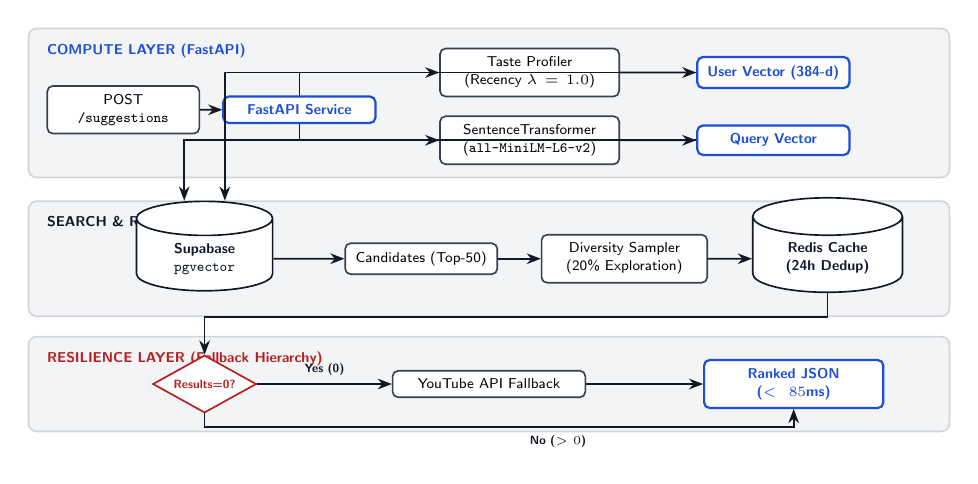
\begin{tikzpicture}[
        scale=0.86, every node/.style={transform shape},
        layer/.style={draw=inkRule, fill=inkLight, rounded corners=3pt, line width=0.6pt},
        block/.style={draw=inkDark, fill=white, rounded corners=2pt, line width=0.6pt, align=center, font=\fontsize{6pt}{7.5pt}\selectfont, inner sep=3.5pt},
        action/.style={draw=focusBlue, fill=white, rounded corners=2pt, line width=0.8pt, align=center, font=\fontsize{6pt}{7.5pt}\selectfont\bfseries\color{focusBlue}, inner sep=3.5pt},
        db/.style={draw=inkBlack, fill=white, cylinder, shape border rotate=90, aspect=0.25, line width=0.6pt, align=center, font=\fontsize{6pt}{7.5pt}\selectfont\bfseries\color{inkBlack}, inner sep=3pt},
        decision/.style={draw=focusRed, fill=white, diamond, aspect=1.8, line width=0.6pt, align=center, font=\fontsize{5pt}{6pt}\selectfont\bfseries\color{focusRed}, inner sep=2pt},
        arr/.style={-{Stealth[length=1.8mm]}, line width=0.6pt, color=inkBlack}
    ]
        % Layer 1
        \draw[layer] (-6.8, 1.3) rectangle (6.8, 3.5);
        \node[anchor=north west, font=\fontsize{6.5pt}{7.5pt}\selectfont\bfseries\color{focusBlue}] at (-6.65, 3.4) {COMPUTE LAYER (FastAPI)};
        \node[block, text width=2.0cm] (req) at (-5.4, 2.3) {POST \texttt{/suggestions}};
        \node[action, text width=2.0cm] (fastapi) at (-2.8, 2.3) {FastAPI Service};
        \node[block, text width=2.4cm] (prof) at (0.6, 2.85) {Taste Profiler\\(Recency $\lambda=1.0$)};
        \node[block, text width=2.4cm] (sbert) at (0.6, 1.85) {SentenceTransformer\\(\texttt{all-MiniLM-L6-v2})};
        \node[action, text width=2.0cm] (uvec) at (4.2, 2.85) {User Vector (384-d)};
        \node[action, text width=2.0cm] (qvec) at (4.2, 1.85) {Query Vector};
        \draw[arr] (req) -- (fastapi);
        \draw[arr] (fastapi) |- (prof);
        \draw[arr] (fastapi) |- (sbert);
        \draw[arr] (prof) -- (uvec);
        \draw[arr] (sbert) -- (qvec);

        % Layer 2
        \draw[layer] (-6.8, -0.75) rectangle (6.8, 0.95);
        \node[anchor=north west, font=\fontsize{6.5pt}{7.5pt}\selectfont\bfseries\color{inkBlack}] at (-6.65, 0.85) {SEARCH \& RANKING ENGINE};
        \node[db, text width=1.8cm] (pgvec) at (-4.2, 0.1) {Supabase\\\texttt{pgvector}};
        \node[block, text width=2.0cm] (cand) at (-1.0, 0.1) {Candidates (Top-50)};
        \node[block, text width=2.2cm] (shuffler) at (2.0, 0.1) {Diversity Sampler\\(20\% Exploration)};
        \node[db, text width=2.0cm] (redis) at (5.0, 0.1) {Redis Cache\\(24h Dedup)};
        \draw[arr] (cand) -- (shuffler);
        \draw[arr] (shuffler) -- (redis);
        \draw[arr] (uvec) -| ($(pgvec.north)+(0.3, 0)$);
        \draw[arr] (qvec) -| ($(pgvec.north)+(-0.3, 0)$);
        \draw[arr] (pgvec) -- (cand);

        % Layer 3
        \draw[layer] (-6.8, -2.45) rectangle (6.8, -1.05);
        \node[anchor=north west, font=\fontsize{6.5pt}{7.5pt}\selectfont\bfseries\color{focusRed}] at (-6.65, -1.15) {RESILIENCE LAYER (Fallback Hierarchy)};
        \node[decision] (check) at (-4.2, -1.75) {Results=0?};
        \node[block, text width=2.6cm] (ytapi) at (0.0, -1.75) {YouTube API Fallback};
        \node[action, text width=2.4cm] (resp) at (4.5, -1.75) {Ranked JSON ($<85$ms)};
        \draw[arr] (redis.south) -- ++(0, -0.35) -| (check.north);
        \draw[arr] (check.east) -- node[above, font=\tiny\bfseries\color{focusRed}]{Yes (0)} (ytapi.west);
        \draw[arr] (check.south) -- ++(0, -0.2) -| node[below, pos=0.3, font=\tiny\bfseries\color{focusBlue}]{No ($>0$)} (resp.south);
        \draw[arr] (ytapi) -- (resp);
    \end{tikzpicture}
\end{frame}

% ==============================================================================
% SLIDE 9: YAMDA PIPELINE DIAGRAM
% ==============================================================================
\begin{frame}{YAMDA-50M Sandbox Pipeline (Samsung PRISM Phase 2)}{Offline research sandbox architecture}
    \begin{columns}[c]
        \begin{column}{0.46\textwidth}
            \centering
            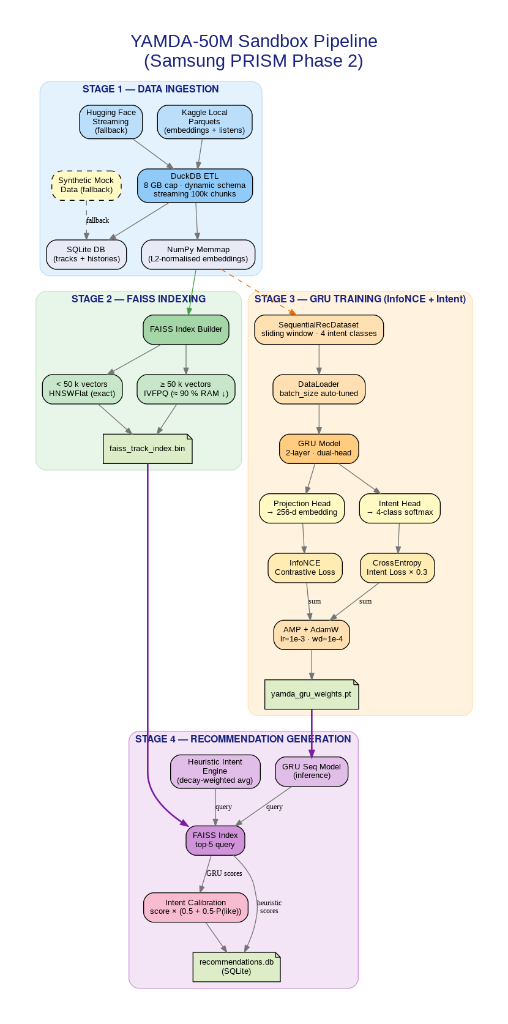
\includegraphics[height=0.72\textheight, keepaspectratio]{figures/yamda_pipeline.png}
        \end{column}

        \begin{column}{0.52\textwidth}
            \begin{block}{Stage 1: Ingestion (\textbf{DuckDB [7]})}
                \fontsize{6.5pt}{8.5pt}\selectfont
                Parquets streamed with 8 GB RAM cap; SQLite stores relations while NumPy Memmap hosts the L2-normalized embedding matrix.
            \end{block}

            \begin{block}{Stage 2: FAISS Indexing (\textbf{IVFPQ [4]})}
                \fontsize{6.5pt}{8.5pt}\selectfont
                Product Quantization compresses $\ge 50$k vectors for 90\% RAM reduction with sub-millisecond retrieval.
            \end{block}

            \begin{block}{Stage 3: Deep GRU Training (\textbf{GRU [1]} / \textbf{PyTorch [8]})}
                \fontsize{6.5pt}{8.5pt}\selectfont
                4-layer GRU with Self-Attention pooling trained via InfoNCE Contrastive + Intent Cross-Entropy loss.
            \end{block}

            \begin{block}{Stage 4: Recommendation Generation}
                \fontsize{6.5pt}{8.5pt}\selectfont
                Calibrates FAISS top-5 ANN queries: $\text{score} \times (0.5 + 0.5 \cdot P(\text{like}))$.
            \end{block}
        \end{column}
    \end{columns}
\end{frame}

% ==============================================================================
% SLIDE 10: DUCKDB ETL BENCHMARKS
% ==============================================================================
\begin{frame}{Work Done: High-Performance ETL Engine (DuckDB [7])}{Analytical ingestion \& relational staging}
    \begin{columns}[T]
        \begin{column}{0.48\textwidth}
            \begin{block}{ETL Architecture}
                \begin{itemize}\small
                    \item \textbf{Disk-Backed Execution:} Enforced an \textbf{8 GB memory ceiling} to prevent OOM errors.
                    \item \textbf{Vectorized Joins:} Joins \texttt{embeddings.parquet} and \texttt{listens.parquet} directly on-disk.
                    \item \textbf{Noise Filtering:} Excluded passive listening records where $\text{played\_ratio\_pct} < 0.15$.
                \end{itemize}
            \end{block}
        \end{column}

        \begin{column}{0.48\textwidth}
            \begin{exampleblock}{Measured Benchmarks}
                \begin{itemize}\small
                    \item \textbf{Catalog Size:} \textbf{156,275 tracks} extracted and indexed.
                    \item \textbf{User Sequences:} \textbf{427 users} parsed with complete chronological logs.
                    \item \textbf{Ingestion Time:} Completed in \textbf{118 seconds}.
                    \item \textbf{RAM Footprint:} Peak execution memory remained below \textbf{450 MB}.
                \end{itemize}
            \end{exampleblock}
        \end{column}
    \end{columns}
\end{frame}

% ==============================================================================
% SLIDE 11: FAISS IVFPQ COMPRESSION & PARAMETER DEFINITIONS
% ==============================================================================
\begin{frame}{Work Done: Vector Quantization (FAISS IVFPQ [4])}{90\% RAM reduction via IVFPQ codebooks}
    \begin{columns}[T]
        \begin{column}{0.49\textwidth}
            \begin{block}{Mathematical Formulation}
                \fontsize{6.8pt}{8.8pt}\selectfont
                $$\mathbf{x} = [\mathbf{x}^{(1)}, \mathbf{x}^{(2)}, \dots, \mathbf{x}^{(m)}] \in \mathbb{R}^D$$
                $$q(\mathbf{x}) = [\mathbf{c}_{i_1}^{(1)}, \mathbf{c}_{i_2}^{(2)}, \dots, \mathbf{c}_{i_m}^{(m)}]$$
                $$d_{ADC}^2(\mathbf{U}, q(\mathbf{w})) = \sum_{j=1}^m \|\mathbf{U}^{(j)} - \mathbf{c}_{i_j}^{(j)}\|_2^2$$
                \textbf{RAM Saving:} $32\text{ B}$ vs $1024\text{ B}$ ($\approx 90\%$ reduction).
            \end{block}
        \end{column}

        \begin{column}{0.49\textwidth}
            \begin{block}{Parameter Definitions}
                \fontsize{6pt}{7.5pt}\selectfont
                \begin{itemize}
                    \item $\mathbf{x} \in \mathbb{R}^D$: High-dimensional track embedding ($D=256$).
                    \item $m = 32$: Number of orthogonal sub-vector slices ($d=D/m=8$).
                    \item $\mathbf{x}^{(j)} \in \mathbb{R}^8$: $j$-th sub-vector component of track $\mathbf{x}$.
                    \item $\mathcal{C}^{(j)}$: Centroid codebook ($k^*=256$, 8-bit quantization per slice).
                    \item $\mathbf{c}_{i_j}^{(j)}$: Nearest centroid vector in codebook $j$ ($i_j \in [0, 255]$).
                    \item $q(\mathbf{x})$: Quantized index represented as a 32-byte code.
                    \item $\mathbf{U} \in \mathbb{R}^{256}$: Unquantized user query profile vector.
                    \item $d_{ADC}^2$: Asymmetric Distance Computation via Look-Up Tables.
                \end{itemize}
            \end{block}
        \end{column}
    \end{columns}
\end{frame}

% ==============================================================================
% SLIDE 12: DEEP GRU v3 HEAVY & PARAMETER DEFINITIONS
% ==============================================================================
\begin{frame}{Work Done: PyTorch [8] GRU [1] v3 Heavy Model Architecture}{3.5M+ parameter sequential recommender}
    \begin{columns}[T]
        \begin{column}{0.50\textwidth}
            \begin{block}{Recurrent Gating Dynamics}
                \fontsize{6.5pt}{8.2pt}\selectfont
                $$\mathbf{z}_t = \sigma(\mathbf{W}_z \mathbf{x}_t + \mathbf{U}_z \mathbf{h}_{t-1} + \mathbf{b}_z)$$
                $$\mathbf{r}_t = \sigma(\mathbf{W}_r \mathbf{x}_t + \mathbf{U}_r \mathbf{h}_{t-1} + \mathbf{b}_r)$$
                $$\tilde{\mathbf{h}}_t = \tanh(\mathbf{W}_h \mathbf{x}_t + \mathbf{U}_h (\mathbf{r}_t \odot \mathbf{h}_{t-1}) + \mathbf{b}_h)$$
                $$\mathbf{h}_t = (1 - \mathbf{z}_t) \odot \mathbf{h}_{t-1} + \mathbf{z}_t \odot \tilde{\mathbf{h}}_t$$
                $$\text{Attention}(\mathbf{Q}, \mathbf{K}, \mathbf{V}) = \text{softmax}\left(\frac{\mathbf{Q}\mathbf{K}^T}{\sqrt{d_k}}\right)\mathbf{V}$$
            \end{block}
        \end{column}

        \begin{column}{0.48\textwidth}
            \begin{block}{Parameter Definitions}
                \fontsize{6pt}{7.5pt}\selectfont
                \begin{itemize}
                    \item $\mathbf{x}_t \in \mathbb{R}^{256}$: Input track embedding at timestep $t \in [1, 20]$.
                    \item $\mathbf{h}_t \in \mathbb{R}^{512}$: Hidden state vector across 4 GRU layers.
                    \item $\mathbf{z}_t \in (0,1)^{512}$: Update gate vector (controls memory retention).
                    \item $\mathbf{r}_t \in (0,1)^{512}$: Reset gate vector (controls history forgetfulness).
                    \item $\tilde{\mathbf{h}}_t$: Candidate hidden state activation via $\tanh$.
                    \item $\mathbf{W}, \mathbf{U}, \mathbf{b}$: Learnable input, recurrent, and bias matrices.
                    \item $\odot$: Element-wise (Hadamard) tensor multiplication.
                    \item $\mathbf{Q}, \mathbf{K}, \mathbf{V}$: Query ($\mathbf{h}_{20}$), Key ($\mathbf{H}$), Value ($\mathbf{H}$) projections ($d_k=128$).
                \end{itemize}
            \end{block}
        \end{column}
    \end{columns}
\end{frame}

% ==============================================================================
% SLIDE 13: MULTI-TASK LOSS & PARAMETER DEFINITIONS
% ==============================================================================
\begin{frame}{Work Done: Contrastive InfoNCE Loss Formulation [3]}{InfoNCE contrastive \& classification loss}
    \begin{columns}[T]
        \begin{column}{0.50\textwidth}
            \begin{block}{Loss Objectives}
                \fontsize{6.8pt}{8.8pt}\selectfont
                $$\mathcal{L}_{\text{InfoNCE}} = -\log \frac{\exp\left(\frac{\mathbf{p} \cdot \mathbf{y}^+}{\tau}\right)}{\exp\left(\frac{\mathbf{p} \cdot \mathbf{y}^+}{\tau}\right) + \sum_{j=1}^{B-1} \exp\left(\frac{\mathbf{p} \cdot \mathbf{y}_j^-}{\tau}\right)}$$
                $$\mathcal{L}_{\text{CrossEntropy}} = -\sum_{c=1}^4 y_c \log \hat{y}_c$$
                $$\mathcal{L}_{\text{joint}} = \mathcal{L}_{\text{InfoNCE}} + 0.3 \cdot \mathcal{L}_{\text{CrossEntropy}}$$
            \end{block}
        \end{column}

        \begin{column}{0.48\textwidth}
            \begin{block}{Parameter Definitions}
                \fontsize{6pt}{7.5pt}\selectfont
                \begin{itemize}
                    \item $\mathbf{p} \in \mathbb{R}^{256}$: L2-normalized predicted embedding from projection head.
                    \item $\mathbf{y}^+ \in \mathbb{R}^{256}$: Ground-truth positive next-track embedding.
                    \item $\mathbf{y}_j^- \in \mathbb{R}^{256}$: In-batch negative samples ($B-1$ sample vectors).
                    \item $\tau$: Learnable temperature parameter (initialized at $\tau_0=0.07$).
                    \item $B$: Batch size ($B=2048$ on CUDA AMP, $B=512$ on CPU).
                    \item $y_c, \hat{y}_c$: Ground truth and predicted logits for 4 intent classes.
                    \item $0.3$: Empirical hyperparameter balancing contrastive and classification loss.
                \end{itemize}
            \end{block}
        \end{column}
    \end{columns}
\end{frame}

% ==============================================================================
% SLIDE 14: UNDERFITTING DIAGNOSIS & RESOLUTION
% ==============================================================================
\begin{frame}{Training Diagnostics: Underfitting Resolution}{Overcoming capacity limits via v3 Heavy}
    \begin{columns}[T]
        \begin{column}{0.48\textwidth}
            \begin{alertblock}{Empirical Diagnosis of 30-Epoch Baseline}
                \begin{itemize}\small
                    \item Initial runs with 2-layer 256-dim GRU yielded:
                    $$\textbf{Epoch 30/30 | Avg Loss: 5.9199}$$
                    $$\text{InfoNCE: } 5.6990, \quad \text{Intent: } 0.7362$$
                    \item \textbf{Root Cause:} The 256-dim backbone lacked expressive capacity for 50M interactions.
                    \item \textbf{Gradient Starvation:} Final-step pooling lost key transitions earlier in the sequence.
                \end{itemize}
            \end{alertblock}
        \end{column}

        \begin{column}{0.48\textwidth}
            \begin{exampleblock}{Architectural Interventions Applied}
                \begin{itemize}\small
                    \item \textbf{4$\times$ Backbone Width:} Scaled hidden dimension from 256 to 512 ($>3.5\text{M}$ params).
                    \item \textbf{Attention Pooling:} Weights critical actions anywhere in history (e.g. LIKE vs SKIP).
                    \item \textbf{Residual Projections:} Skip connections ensure direct gradient flow to early cells.
                    \item \textbf{Cosine Annealing:} Bypasses local plateaus.
                \end{itemize}
            \end{exampleblock}
        \end{column}
    \end{columns}
\end{frame}

% ==============================================================================
% SLIDE 15: EMPIRICAL TRAINING DYNAMICS GRAPH
% ==============================================================================
\begin{frame}{Empirical Training Dynamics: GRU Convergence Curve}{Trajectory \& hyperparameter validation}
    \begin{columns}[c]
        \begin{column}{0.52\textwidth}
            \centering
            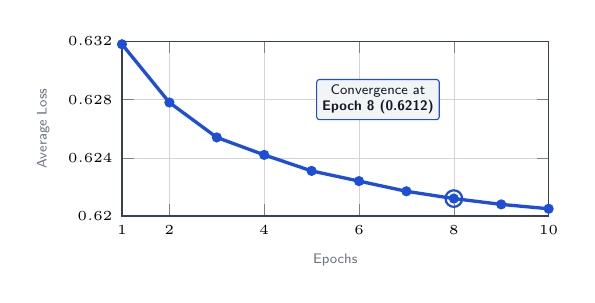
\begin{tikzpicture}
                \begin{axis}[
                    width=7.0cm, height=3.8cm,
                    xlabel={\fontsize{5.5pt}{6.5pt}\selectfont Epochs},
                    ylabel={\fontsize{5.5pt}{6.5pt}\selectfont Average Loss},
                    xmin=1, xmax=10,
                    ymin=0.6200, ymax=0.6320,
                    xtick={1, 2, 4, 6, 8, 10},
                    ytick={0.6200, 0.6240, 0.6280, 0.6320},
                    y tick label style={/pgf/number format/fixed, /pgf/number format/precision=4, font=\fontsize{5pt}{6pt}\selectfont},
                    grid=both, grid style={line width=0.2pt, draw=inkRule},
                    tick label style={font=\fontsize{5pt}{6pt}\selectfont},
                    label style={font=\fontsize{5.5pt}{6.5pt}\selectfont\color{inkMuted}},
                    axis line style={inkDark, line width=0.5pt}
                ]
                    \addplot[color=focusBlue, mark=*, mark size=1.2pt, line width=1.2pt] coordinates {
                        (1, 0.6318) (2, 0.6278) (3, 0.6254) (4, 0.6242) (5, 0.6231)
                        (6, 0.6224) (7, 0.6217) (8, 0.6212) (9, 0.6208) (10, 0.6205)
                    };
                    \draw[focusBlue, line width=0.8pt] (axis cs:8, 0.6212) circle (3pt);
                    \node[draw=focusBlue, fill=inkLight, rounded corners=1pt, font=\fontsize{4.8pt}{5.8pt}\selectfont, align=center, text=inkBlack, inner sep=2pt] 
                        at (axis cs:6.4, 0.6280) {Convergence at\\\textbf{Epoch 8 (0.6212)}};
                \end{axis}
            \end{tikzpicture}
        \end{column}

        \begin{column}{0.44\textwidth}
            \begin{block}{Configured Hyperparameters}
                \fontsize{6pt}{8pt}\selectfont
                \begin{tabular}{ll}
                    \toprule
                    \textbf{Component} & \textbf{Production Value} \\
                    \midrule
                    Backbone & 4-Layer GRU (512-d) \\
                    Attention Heads & 4 Heads ($\text{embed}=512$) \\
                    Sequence Length & $T = 20$ Interactions \\
                    Batch Size & 2048 (CUDA AMP) / 512 (CPU) \\
                    Base LR & $3 \times 10^{-3}$ (AdamW) \\
                    Schedulers & 5-epoch Warmup + Cosine \\
                    Temperature $\tau$ & Learnable (init $0.07$) \\
                    Checkpoints & Every 15 Epochs \\
                    \bottomrule
                \end{tabular}
            \end{block}
        \end{column}
    \end{columns}
\end{frame}

% ==============================================================================
% SLIDE 16: LONG-HORIZON CHECKPOINTING
% ==============================================================================
\begin{frame}{Work Done: Long-Horizon Checkpoint Engine}{Decoupled multi-session persistence}
    \begin{columns}[T]
        \begin{column}{0.48\textwidth}
            \begin{block}{Long-Horizon Training Requirements}
                \begin{itemize}\small
                    \item Training a 3.5M parameter network on 50M records requires extended multi-stage execution.
                    \item Training sessions must be resilient to runtime interruptions and system preemption.
                    \item Uncheckpointed training risks loss of progress and model state degradation.
                \end{itemize}
            \end{block}
        \end{column}

        \begin{column}{0.48\textwidth}
            \begin{exampleblock}{Engineered Auto-Resume Logic}
                \begin{itemize}\small
                    \item \textbf{15-Epoch Checkpointing:} Automatically saves full state dicts at epochs 15, 30, 45, and 60.
                    \item \textbf{State Persistence:} Preserves:
                    $$\langle \mathbf{W}_{\text{model}}, \mathbf{S}_{\text{optimizer}}, \mathbf{S}_{\text{scheduler}}, \mathbf{S}_{\text{scaler}}, \log \tau \rangle$$
                    \item \textbf{Zero-Intervention Resume:} Auto-loads from \texttt{yamda\_checkpoint.pt} and seamlessly resumes training.
                \end{itemize}
            \end{exampleblock}
        \end{column}
    \end{columns}
\end{frame}

% ==============================================================================
% SLIDE 17: EMPIRICAL CASE STUDY
% ==============================================================================
\begin{frame}{Empirical Results: Test User Case Study}{Comparative next-item predictions}
    \centering
    \fontsize{6pt}{7.5pt}\selectfont
    \renewcommand{\arraystretch}{1.2}
    \resizebox{\textwidth}{!}{%
    \begin{tabular}{l l l l}
        \toprule
        \rowcolor{inkDark}
        \textbf{\color{white}User ID} & 
        \textbf{\color{white}Input History Sequence ($T=5$)} & 
        \textbf{\color{white}GRU Recommender Top 5 (Deep)} & 
        \textbf{\color{white}Heuristic Engine Top 5 (Recency)} \\
        \midrule
        \rowcolor{inkLight}
        \textbf{User 100} & 
        \texttt{[3175251, 1299533, 7415847, 6870586, 4734787]} & 
        \texttt{[3443475, 6060302, 4531263, 4805129, 2413614]} & 
        \texttt{[\textbf{4734787}, 3426714, 5150945, 451318, 2077046]} \\
        \rowcolor{white}
        \textbf{User 200} & 
        \texttt{[2859641, 2943786, 4117955, 5134208, \textbf{3778807}]} & 
        \texttt{[\textbf{\color{focusBlue}5811656}, 4219887, 3361052, 1252472, \textbf{3778807}]} & 
        \texttt{[\textbf{\color{focusBlue}3778807}, 3741007, 1346490, 5541739, \textbf{5811656}]} \\
        \bottomrule
    \end{tabular}%
    }

    \vspace{0.3cm}
    \begin{columns}[T]
        \begin{column}{0.48\textwidth}
            \begin{block}{Heuristic Recency Engine Behavior}
                \small Directly surfaces recent \textbf{historical tracks} (e.g., track \textbf{3778807} for User 200), prioritizing immediate session mood continuity.
            \end{block}
        \end{column}
        \begin{column}{0.48\textwidth}
            \begin{block}{Deep GRU Model Behavior}
                \small Infers broader \textbf{latent relationships} (e.g., discovering track \textbf{5811656}), uncovering non-linear semantic transitions.
            \end{block}
        \end{column}
    \end{columns}
\end{frame}

% ==============================================================================
% SLIDE 18: RESILIENCE & FALLBACK HIERARCHY
% ==============================================================================
\begin{frame}{Work Done: 4-Tier Resilience \& Anti-Repetition Cache}{Deterministic 100\% fulfillment cascade}
    \centering
    \fontsize{6pt}{8pt}\selectfont
    \renewcommand{\arraystretch}{1.25}
    \resizebox{\textwidth}{!}{%
    \begin{tabular}{l l l}
        \toprule
        \rowcolor{inkDark}
        \textbf{\color{white}Tier} & \textbf{\color{white}Method} & \textbf{\color{white}Trigger Condition \& Latency Budget} \\
        \midrule
        \rowcolor{inkLight}
        \textbf{\color{focusBlue}Tier 1} & \textbf{Semantic Match} & \textbf{Preferred method;} $D_C(\mathbf{U}, \mathbf{w}) \le 0.28$ via Supabase \texttt{pgvector} HNSW index ($<45\text{ ms}$). \\
        \textbf{Tier 2} & \textbf{Metadata Heuristic} & \textbf{Triggered if vector search yields 0 results;} exact genre match from catalog SQLite ($<15\text{ ms}$). \\
        \rowcolor{inkLight}
        \textbf{Tier 3} & \textbf{Genre Trending} & \textbf{Triggered if local metadata fails;} live query to YouTube Data API V3 in genre ($<120\text{ ms}$). \\
        \textbf{\color{focusRed}Tier 4} & \textbf{Global Trending} & \textbf{Ultimate fallback;} retrieves live top global charts to eliminate empty query errors ($<90\text{ ms}$). \\
        \bottomrule
    \end{tabular}%
    }

    \vspace{0.3cm}
    \begin{columns}[T]
        \begin{column}{0.48\textwidth}
            \begin{block}{Redis Deduplication Cache}
                \small 24-hour sliding-window filter excludes recently suggested IDs, completely eliminating song fatigue.
            \end{block}
        \end{column}
        \begin{column}{0.48\textwidth}
            \begin{block}{Diversity Sampler}
                \small Injects 20\% exploration tracks from the top-50 pool using Gibbs sampling to shatter filter bubbles.
            \end{block}
        \end{column}
    \end{columns}
\end{frame}

% ==============================================================================
% SLIDE 19: PRODUCTION FASTAPI CONTRACT
% ==============================================================================
\begin{frame}[fragile]{Work Done: Production FastAPI Service}{Real-time lifecycle \& verified JSON contract}
    \begin{columns}[T]
        \begin{column}{0.48\textwidth}
            \begin{block}{Verified Request: \texttt{POST /suggestions}}
                \fontsize{6pt}{7.5pt}\selectfont\ttfamily
                \{\\
                \quad "user\_id": "user@example.com",\\
                \quad "songs": ["Shape of You - Ed Sheeran"],\\
                \quad "genre": "Pop"\\
                \}
            \end{block}

            \begin{block}{Execution Lifecycle}
                \begin{enumerate}\fontsize{6pt}{8pt}\selectfont
                    \item JWT Authentication (\texttt{get\_current\_user}).
                    \item In-memory profile calculation ($<1.2\text{ ms}$).
                    \item \texttt{pgvector} Cosine distance lookup ($<45\text{ ms}$).
                    \item Redis 24hr deduplication filter.
                    \item Background task logging to PostgreSQL.
                \end{enumerate}
            \end{block}
        \end{column}

        \begin{column}{0.48\textwidth}
            \begin{block}{Verified Response Payload}
                \fontsize{6pt}{7.5pt}\selectfont\ttfamily
                \{\\
                \quad "status": "success",\\
                \quad "source": "semantic\_search",\\
                \quad "results": [\\
                \quad\quad \{\\
                \quad\quad\quad "title": "Perfect",\\
                \quad\quad\quad "artist": "Ed Sheeran",\\
                \quad\quad\quad "score": 0.89\\
                \quad\quad \},\\
                \quad\quad \{\\
                \quad\quad\quad "title": "Someone You Loved",\\
                \quad\quad\quad "artist": "Lewis Capaldi",\\
                \quad\quad\quad "score": 0.85\\
                \quad\quad \}\\
                \quad ]\\
                \}
            \end{block}
        \end{column}
    \end{columns}
\end{frame}

% ==============================================================================
% SLIDE 20: ROADMAP & REFERENCES
% ==============================================================================
\begin{frame}{Project Deliverables Summary \& Academic References}{IEEE bibliographic foundation \& review summary}
    \begin{columns}[T]
        \begin{column}{0.44\textwidth}
            \begin{exampleblock}{Review 1 Deliverables Completed}
                \begin{itemize}\fontsize{5.8pt}{7.5pt}\selectfont
                    \item DuckDB ETL processing 156k tracks in 118 seconds.
                    \item FAISS IVFPQ index achieving 90\% RAM compression.
                    \item PyTorch GRU v3 Heavy (3.5M params) architecture.
                    \item 15-epoch auto-resume checkpointing engine.
                    \item Live FastAPI service with pgvector and Redis cache.
                \end{itemize}
            \end{exampleblock}

            \begin{block}{Phase 2 Roadmap}
                \begin{itemize}\fontsize{5.8pt}{7.5pt}\selectfont
                    \item Execute 60-epoch training to convergence.
                    \item Deploy GRU inside FastAPI for live A/B testing.
                    \item Index full 50M YAMDA catalog via distributed FAISS.
                \end{itemize}
            \end{block}
        \end{column}

        \begin{column}{0.54\textwidth}
            \begin{block}{Academic References (IEEE Format)}
                \fontsize{4.4pt}{5.4pt}\selectfont
                \begin{enumerate}\setlength{\itemsep}{1.2pt}\setlength{\parskip}{0pt}\leftmargin=6pt
                    \item[{[1]}] B. Hidasi \textit{et al.}, ``Session-based recommendations with recurrent neural networks,'' in \textit{Proc. 4th Int. Conf. Learn. Represent. (ICLR)}, 2016. \href{https://arxiv.org/abs/1511.06939}{\color{focusBlue}{[arXiv:1511.06939]}}
                    \item[{[2]}] N. Reimers and I. Gurevych, ``Sentence-BERT: Sentence embeddings using siamese BERT-networks,'' in \textit{Proc. Conf. EMNLP}, 2019, pp. 3982--3992. \href{https://arxiv.org/abs/1908.10084}{\color{focusBlue}{[arXiv:1908.10084]}}
                    \item[{[3]}] A. van den Oord, Y. Li, and O. Vinyals, ``Representation learning with contrastive predictive coding,'' \textit{arXiv preprint arXiv:1807.03748}, 2018. \href{https://arxiv.org/abs/1807.03748}{\color{focusBlue}{[arXiv:1807.03748]}}
                    \item[{[4]}] J. Johnson, M. Douze, and H. J{\'e}gou, ``Billion-scale similarity search with GPUs,'' \textit{IEEE Trans. Big Data}, vol. 7, no. 3, pp. 535--547, 2021. \href{https://arxiv.org/abs/1702.08734}{\color{focusBlue}{[IEEE/arXiv:1702.08734]}}
                    \item[{[5]}] M. Spi{\v{s}}{\'a}k \textit{et al.}, ``Scalable approximate nonsymmetric autoencoder for collaborative filtering,'' in \textit{Proc. 17th ACM RecSys}, 2023, pp. 838--844. \href{https://arxiv.org/abs/2308.06733}{\color{focusBlue}{[RecSys/arXiv:2308.06733]}}
                    \item[{[6]}] P. Loshkin, ``YAMDA: Yet another music dataset,'' \textit{GitHub repository / Hugging Face}, 2023. \href{https://github.com/ploshkin}{\color{focusBlue}{[Online Dataset]}}
                    \item[{[7]}] M. Raasveldt and H. M{\"u}hleisen, ``DuckDB: An embeddable analytical database,'' in \textit{Proc. ACM SIGMOD}, 2019, pp. 1981--1984. \href{https://doi.org/10.1145/3299869.3320212}{\color{focusBlue}{[ACM SIGMOD]}}
                    \item[{[8]}] A. Paszke \textit{et al.}, ``PyTorch: An imperative style, high-performance deep learning library,'' in \textit{Adv. Neural Inf. Process. Syst. 32 (NeurIPS)}, 2019, pp. 8024--8035. \href{https://arxiv.org/abs/1912.01703}{\color{focusBlue}{[NeurIPS/arXiv]}}
                \end{enumerate}
            \end{block}

            \vspace{0.08cm}
            \centering
            \textbf{\fontsize{6.5pt}{7.5pt}\selectfont\color{focusBlue}Thank You \textbar\ Questions \& Technical Discussion}
        \end{column}
    \end{columns}
\end{frame}

\end{document}
